\documentclass[a4paper, 11pt, table]{article}
\usepackage[english]{babel}
\usepackage[utf8]{inputenc} % can't use utf8x with biblatex from apa7
\usepackage{comment}
\usepackage{lipsum}
% \usepackage{fullpage}
\usepackage{amsmath}
\usepackage{graphicx}
\usepackage{enumitem}
\usepackage{listings}
\usepackage{verbatim}
\usepackage{eurosym}
\usepackage[export]{adjustbox}
\usepackage[a4paper, total={6.7in, 9in}]{geometry} % make the pages wider
\usepackage{ragged2e} % add the ability to justify text
\usepackage{gensymb}  % for \degree
\usepackage{physics}
\usepackage{wasysym}
\usepackage{float}
\usepackage{url}
\usepackage[citestyle=numeric, sorting=none]{biblatex}
\usepackage{csquotes}
\usepackage{hyperref}
\hypersetup{
    colorlinks=true,
    linkcolor=blue,
    filecolor=blue,      
    urlcolor=cyan,
    citecolor=blue,
    pdftitle={Gamma spectroscopy}
}
\usepackage[capitalize]{cleveref}
\addbibresource{bibliography.bib}
% \usepackage[nottoc]{tocbibind}
\usepackage{multicol}
\usepackage{multirow}
\usepackage{wrapfig}
\usepackage{subcaption} % mosaic of figures 
\usepackage{mwe}
\usepackage{bm}
\usepackage{siunitx}
\sisetup{separate-uncertainty=true}
\usepackage{standalone}
\usepackage{tikz}
\usepackage[version=4]{mhchem}
\usepackage{booktabs}


\captionsetup{tableposition=bottom, figureposition=bottom}
\captionsetup[figure]{labelfont={bf, small}, textfont={small, sl}}
\captionsetup[table]{labelfont={bf, small}, textfont={sl, small}, position=top}

\graphicspath{{images/}}

\usepackage{titlesec}
\setlength{\parindent}{0pt}
%\setlength{\parskip}{0.8em}
%\titlespacing*{\section}      {0em}{0em}{0em}
%\titlespacing*{\subsection}   {0em}{0em}{0em}

\usepackage{longtable} % table across multiple pages
\usepackage{caption}

\begin{document}

\begin{titlepage}

    \newcommand{\HRule}{\rule{\textwidth}{0.5mm}} % Defines a new command for the horizontal lines, change thickness here

    \center % Center everything on the page

    %----------------------------------------------------------------------------------------
    %    HEADING SECTIONS
    %----------------------------------------------------------------------------------------

    \textsc{\LARGE University of Groningen}\\[1.5cm] % Name of your university/college
    \textsc{\Large Physics Laboratory 4}\\[0.5cm] % Major heading such as course name
    %\textsc{\large Assignment 1}\\[0.5cm] % Minor heading such as course title

    %----------------------------------------------------------------------------------------
    %    TITLE SECTION
    %----------------------------------------------------------------------------------------

    \HRule \\[0.4cm]
    { \huge \bfseries Gamma Ray Spectroscopy (GMA)}\\[0.3cm] % Title of your document
    { \Large \bfseries Calibration of a SiPM spectrometer and determination \\of its resolution and efficiency at different energies}\\[0.3cm] % Title of your document
    \HRule \\[1.5cm]

    %----------------------------------------------------------------------------------------
    %    AUTHOR SECTION
    %----------------------------------------------------------------------------------------

    \begin{minipage}{0.4\textwidth}
        \begin{flushleft} \large
            \emph{Authors:}\\
            Nicol\'{o} \textsc{Montalti} \textit{(s4947231)} \\
            Anna F. \textsc{Esselink} \textit{(s4149653)} \\
        \end{flushleft}
    \end{minipage}
    ~
    \begin{minipage}{0.4\textwidth}
        \begin{flushright} \large
            \emph{Course Coordinaters:} \\
            Aleksandra Biegun\\
            Eifion Prinsen\\
            \emph{Teaching Assistant:}\\
            Adrian Sidhu
            \hfill \\
        \end{flushright}
    \end{minipage}\\[1cm]

    % If you don't want a supervisor, uncomment the two lines below and remove the section above

    %\Large \emph{Author:}\\
    %John \textsc{Smith}\\[3cm] % Your name

    %----------------------------------------------------------------------------------------
    %    DATE SECTION
    %----------------------------------------------------------------------------------------

    {\large \today}\\[1cm] % Date, change the \today to a set date if you want to be precise

    %----------------------------------------------------------------------------------------
    %    LOGO SECTION
    %----------------------------------------------------------------------------------------

    %\includegraphics[width=300px, keepaspectratio]{Images/prettyfrontpagepicture.jpg}\\[1cm] % Include a department/university logo - this will require the graphicx package
    %\caption{}



    \begin{abstract}
        \noindent Gamma rays are typically originated from the decay of radioactive nuclei. Analysing the spectrum of a source is often useful to identify it, especially in astronomy. In this experiment, the spectra of Am-241, Co-60, Cs-137, and Na-22 were analysed with a silicon photomultiplier (SiPM). Together with the SiPM, BGO, CsI, and LYSO crystals were used. The optimal threshold voltage of each crystal was found, the spectrometer was calibrated and the efficiency and the resolution were determined. The efficiency and the resolution were found to decrease with energy. The calibration factors were found to be inversely proportional to the light yield of the crystal. A new set of measurements, with different settings, could improve the precision of the results. A more precise behavior of the resolution and the efficiency at different energies could be determined.
    \end{abstract}

    %----------------------------------------------------------------------------------------

    \vfill % Fill the rest of the page with whitespace

\end{titlepage}
\newgeometry{textwidth=5.875in,textheight=9.1in}

%\tableofcontents
\begingroup
\hypersetup{linkcolor=black}
\setlength{\parskip}{0em}
\par
\tableofcontents
\endgroup
\newpage

\section{Introduction}
%basically paraphrasing the introduction from the manual:

%what are gamma rays
Gamma rays can be found on the extreme high energy and short wavelength end of the electromagnetic spectrum. Most gamma radiation originates from the decay of radioactive nuclei. These type of gamma rays have an energy ranging from 100 keV to 8 MeV, where the latter corresponds to the approximate binding energy of individual nucleons. The energy and number of the gamma ray photons that are emitted are dependent on certain characteristics of the nuclei, hence gamma ray spectroscopy can be used to identify radioactive nuclei. Highly energetic astronomical objects, like pulsars, quasars, and supernovae can produce gamma rays of higher energies into the TeV range. These high energy gamma rays are often created through bremsstrahlung \cite{meyers_gamma-ray_2003}.\\

%how/when where they discovered
In 1900 physicist Paul Villard discovered gamma rays when he was examining the $\beta$ decay from radium samples. During this, he discovered another type of radiation, with significantly higher penetration. The radiation was later named gamma rays by Ernest Rutherford, who also named alpha and beta rays, based on their penetrability. It was not until 1914, that it was discovered by Rutherford, that gamma rays, unlike alpha and beta rays, do not have a mass and are instead a form of electromagnetic radiation. This was proven by showing that gamma rays are reflected by crystal surfaces \cite{lannunziata_radioactivity_2007}.\\

%source: book, radioactivity: introduction and history

%aim of the experiment & short description of experiment
This experiment will focus on gamma ray spectroscopy. The gamma spectrum of several radioactive sources will be measured using a silicon photomultiplier (SiPM) spectrometer. The scintillation detector of the spectrometer has different scintillation crystals with varying properties. The ideal threshold voltage and the corresponding detection efficiency and signal-to-noise ratio will be determined for each crystal. After this, the spectra will be calibrated, and the resolution of each peak will be determined.

\section{Theory}
% relatively short, most of the relevant theory is in the experimental set up/ procedure
In this paper, we will focus on gamma rays emitted in the decay of radioactive nuclei. To allow this decay to happen, the nuclei need to be in an excited state. They will transition to the ground state by emitting a photon (gamma ray):
\begin{equation}
    \ce{^A_ZX^* -> ^A_ZX + \gamma}
\end{equation}
Energy $E_\gamma$ of the gamma ray is given by the energy difference between the initial $E_i$ and final $E_f$ state:
\begin{equation} \label{eq:energy_gammaray}
    E_\gamma = E_i -E_f = h\nu
\end{equation}
$\alpha$ or $\beta$ decay often precede $\gamma$ decay, because as the daughter nuclei of both reactions are often in an excited state. \cite{cottingham_2004_an}\\

The rate at which unstable nuclei decay is dependent on their half-life $T_{1/2}$, which is defined as the time it takes half of the original number of radioactive nuclei to decay. The number of unstable nuclei over time is given by:
\begin{equation}
    N(t) = N_0 e^{-\lambda t}
\end{equation}
Where $N_0$ is the number of radioactive nuclei at $t=0$ and $\lambda$ is the decay constant defined as: $\lambda = \frac{\ln{2}}{T_{1/2}}$. Next the activity $A$, the number of decays per second, can be defined as: $A = \lambda N$. \cite{cottingham_2004_an} Consequently the activity will decrease at the same rate as $N$, where this time $A_0$ is the activity at $t=0$:
\begin{align} \label{eq:activity}
    A(t) & = A_0 \cdot e^{-\lambda t} \nonumber                \\
         & = A_0 \cdot e^{-\frac{\ln{2}}{T_{1/2}} t} \nonumber \\
         & = A_0 \cdot 2^{-\frac{t}{T_{1/2}}}
\end{align}

%question 3 from manual, should maybe be in appendix?
One example of $\beta$ decay followed by $\gamma$ decay is the decay of $\ce{^{60}Co}$. Its daughter nuclei $\ce{^{60}Ni}$ ends up in an excited state after the $\beta$ decay, and transitions to the ground state through the emissions of two $\gamma$ rays.
\begin{equation} \label{eq:Co_decay}
    \ce{^{60}_{27}Co -> ^{60}_{28}Ni + e^- + \Bar{\nu_e} + 2\gamma}
\end{equation}

The available energy can be determined by the difference of the nuclear masses:
\begin{align*}
    Q & = [M(\ce{^{60}Co})  - M(\ce{^{60}Ni})]\cross 931.494 \mathrm{MeV/c^2} \\
      & = (59.933816 - 59.930785)\cross 931.494 = 2.823 MeV
\end{align*}
Given that the intermediate state has an energy of 1.332 MeV, the energy of the first emitted $\gamma$ ray is 1.173 MeV and the second one 1.332 MeV. Based on \cref{eq:energy_gammaray}, the corresponding frequencies are $2.84\cdot 10^{20}$ Hz and $3.22\cdot 10^{20}$ Hz respectively.\\
The other three sources used in the experiment, Am-241, Cs-137 and Na-22, have gamma ray energies of 59.5 keV, 661.7 keV and 1275.0 keV respectively.\cite{heath_scintillation_1964}

%PER DECAY OF CO-60, 2 gamma rays emitted, if the half-life of Ni-60 is much shorter than CO-60, then to find efficiency we need to divide found frequency by 2?



\section{Experimental set-up and measuring process}
\subsection{Experimental set-up}
The experimental setup consists of four main components: a Power Supply and Amplification Unit (PSAU - SP5600), a Desktop Digitizer (DT5720A), a Splitter (A315), and a Mini Spectrometer (SP5606). The components are connected as shown in figure \ref{fig:setup}. \\

The mini spectrometer works through scintillation detection. The basic principle of scintillation detectors is the process of solid material, being excited by radiation, after which it emits light. The number of photons that are absorbed by the material is proportional to the number of photons emitted. The photons are collected by a photo-cathode, which in turn emits electrons. The pulses are proportional to the energy that was produced. The photomultiplier amplifies these electric pulses, after which they can be detected. \cite{KRAMAR19992467}\\

In this experiment, three different scintillating crystals were used: caesium iodide (CsI), lutetium–yttrium oxyorthosilicate (LYSO), and bismuth germanate (BGO).\\

% source: https://www.sciencedirect.com/topics/engineering/scintillation-detector#:~:text=Scintillation%20detectors%20are%20used%

%The spectrometer uses a silicon photomultiplier (SiPM). How does this operate and how does it compare to a photomultiplier tube (PMT)?
The spectrometer used in the experiment is a silicon photomultiplier (SiPM), which is the component that produces the electric pulses as a response to absorbing photons. A pulse is generally tens of nanoseconds long and contains $10^5$ to $10^6$ electrons, which implies a high gain.
The structure of a SiPM is an arrangement of thousands of in parallel connected microcells which consist of an avalanche photodiode (APD) and a quenching resistor. The ADP operates in Geiger mode, which means they operate on a voltage above the breakdown threshold voltage, which is the level at which an electron or hole can trigger an avalanche. The threshold voltage can be altered during the experiment to change the count rate. An increase in the threshold voltage results in a decrease of the count rate. The ADP is put back in the Geiger mode by the quenching resistor \cite{kk_2016_what}.\\
%source: https://hub.hamamatsu.com/jp/en/technical-note/how-sipm-works/index.html

Compared to the traditional photomultiplier tube (PMT), the SiPM has a similar gain and photodetection efficiency. However, the SiPM does have a lower excess noise factor and needs fewer photons to obtain the same signal-to-noise ratio. Other advantages of the SiPM compared to the PMT is that it has an immunity to magnetic fields, allowing it to operate in strong magnetic fields; it operates on a lower voltage and is smaller in size. \cite{WAGATSUMA2017203}\\

%In gamma scintillation detectors, the counts are not plotted directly against the energy, but instead ADC channels. What is an ADC channel and how does it relate to the energy of the detector?
%Why does the detector record in ADC channels and not energies???
The measurements taken by the scintillation detector will be presented as the number of counts per analog-to-digital converter (ACD) channels. Each channel represents a specific range of energy in the spectrum. The number of counts in each channel represents the intensity of the radiation in that energy range. The reason that the detector displays the ADC channels instead of plotting the counts directly against energy, is because the conversion factor between channels and energy will differ between different crystals and threshold voltages.


%figure of experimental setup including mini spectrometer
\begin{figure} [h!]
    \centering
    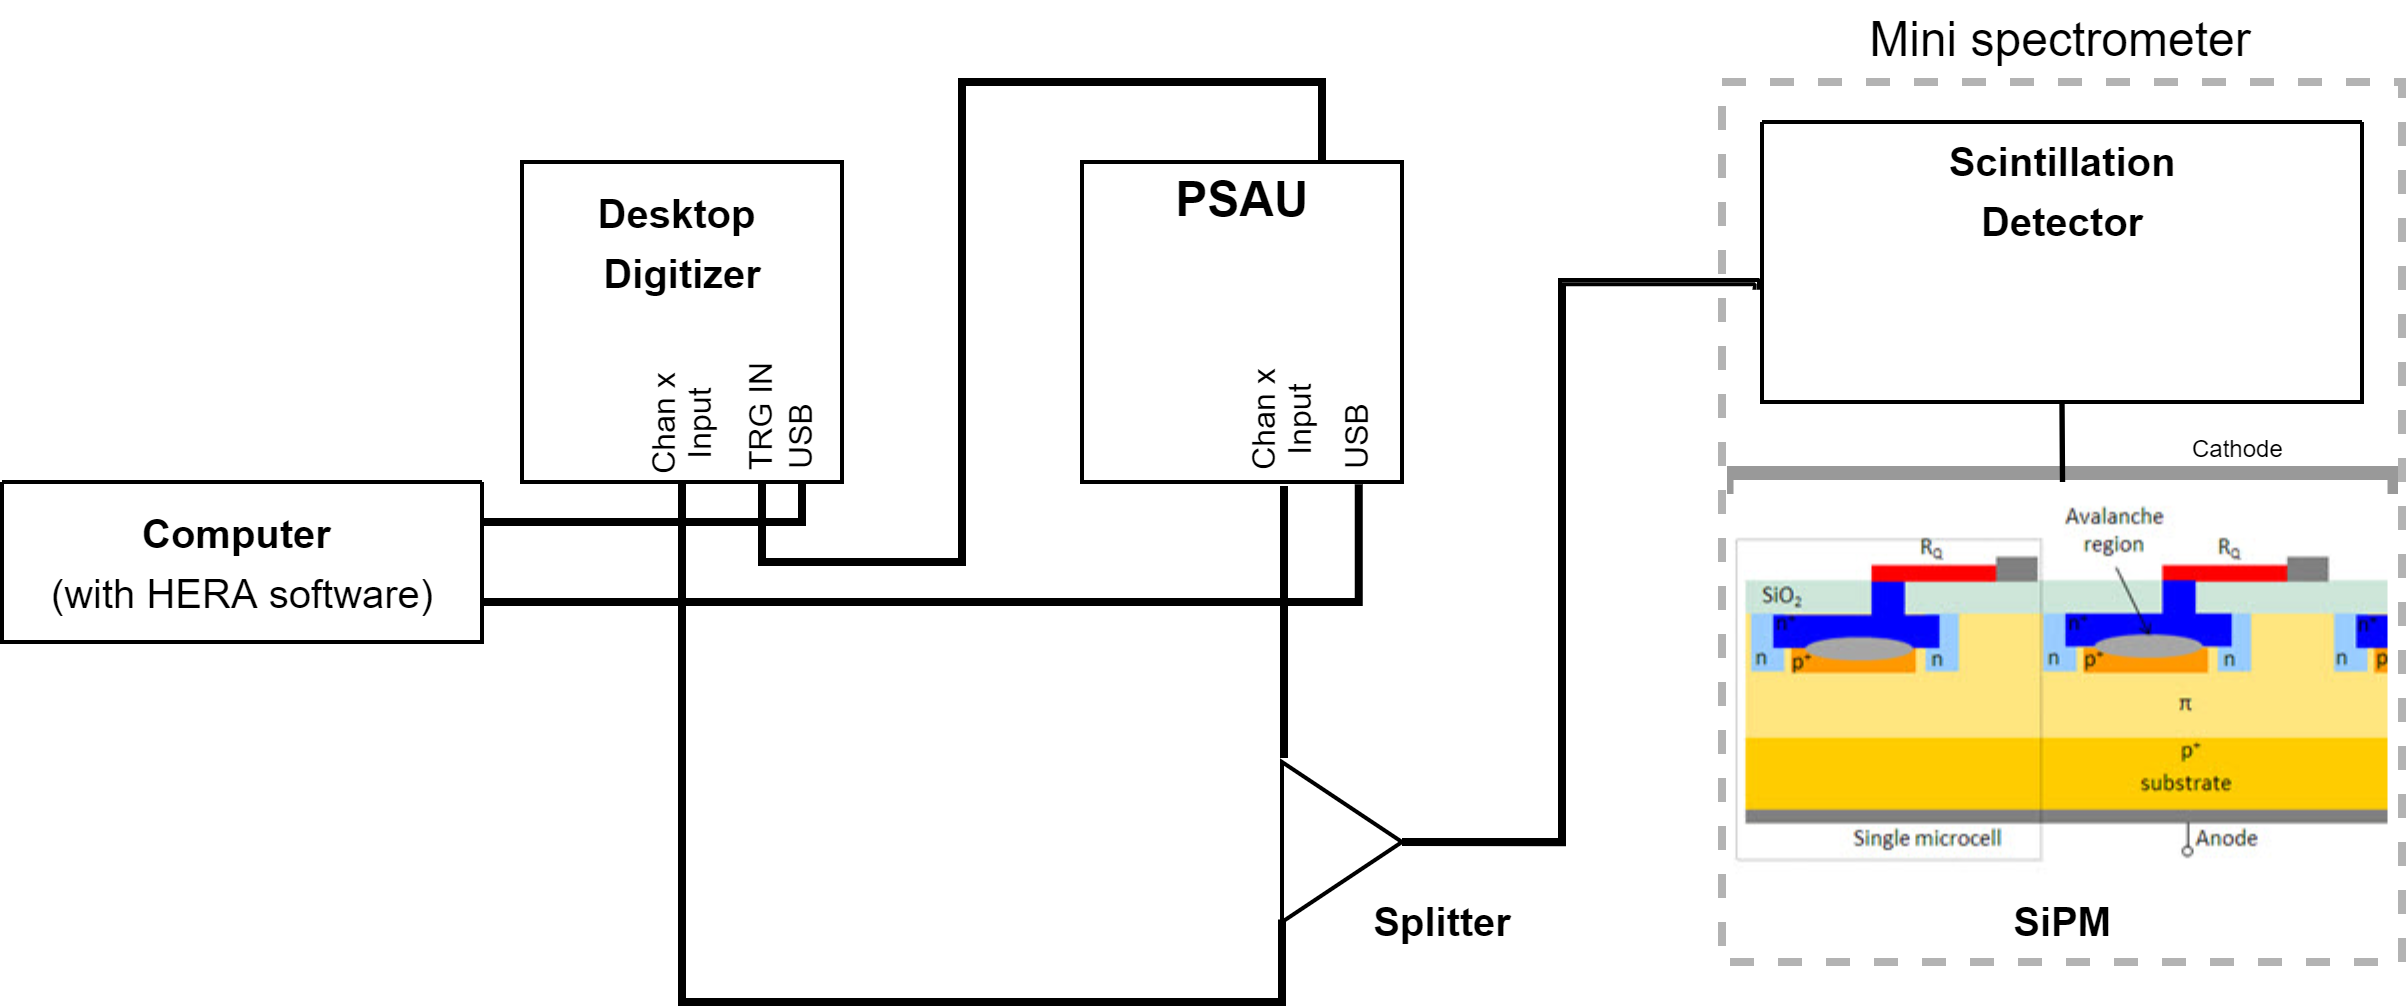
\includegraphics[width=0.98\textwidth]{figures/exp_setup_GMA.png}
    \caption{Circuit of the experimental setup with a diagram of the spectrometer. Gamma rays from the source will hit the scintillation detector, which in turn emits lower energy photons that are detected by the photocathode of the SiPM. Only 2 microcells of the SiPM are shown. This signal from the anode goes back to the computer. (SiPM diagram from \cite{kk_2016_what})}%will add more info later
    \label{fig:setup}
\end{figure}


\subsection{Measuring process}
\paragraph{Threshold optimization}
In order to determine the optimal threshold potential for each crystal, the frequency of gamma ray detection was measured for different thresholds. The measurement was performed both with and without a source for each crystal. The sources used were Am-241, Co-60, Cs-137, and Na-22. The frequency was expected to decrease with the increasing of the threshold both with and without a source. The signal-to-noise ratio (SNR) was computed by dividing the frequency of detected gamma rays with a source by the frequency without a source. The optimal threshold energy was then found maximizing the SNR.

\paragraph{Efficiency}
At the chosen threshold energy, the efficiency of the detector was then evaluated. The absolute efficiency $\epsilon_0$ is defined as the number of detected gamma rays over the total number of emitted gamma rays per unit of time
\begin{equation} \label{eq:efficiency}
    \epsilon_0 = \frac{N_\text{detected}}{N_\text{total}}
\end{equation}
It is also possible to define an intrinsic efficiency $\epsilon_1$ as the number of detected gamma rays over the incident gamma rays
\begin{equation} \label{eq:intrinsic_efficiency}
    \epsilon_1 = \frac{N_\text{detected}}{N_\text{incident}}
\end{equation}
Supposing that exactly half of the gamma rays are emitted in the direction of the detector, $N_\text{incident}$ can be approximated as $N_\text{total} / 2$, and so $\epsilon_1 \approx 2\epsilon_0$.\\

The number of emitted gamma rays per unit of time was found from the activity of the nuclei. All the nuclei but Co-60 emit one gamma ray per decay, so the frequency of the gamma ray emission is equal to the activity of the nuclei. Co-60 emits two gamma rays per decay and so the frequency of emission is the double of the activity. The activities of the sources on the day of the experiment were found from some known initial activity applying the radioactive decay law (\cref{eq:activity})

\paragraph{Calibration}
Spectrometers return spectra expressed in counts per channel. In order to have information about the energy of an unknown spectrum, the instrument must be calibrated. The calibration was performed using the same sources used to determine the thresholds: Am-241, Co-60, Cs-137 and Na-22. The system was calibrated independently for each crystal. For each source, a spectrum was recorded and compared with the values found in literature \cite{heath_scintillation_1964}. The peaks were identified with the help of a signal analysis library \cite{2020SciPy-NMeth} and associated with their known energies. Finally, peaks' energies were plotted against channels. A linear fit returned the conversion factors. The conversion factors of the crystals were then compared with their light yield to determine the relationship between these two quantities.

\paragraph{Resolution}
The energy resolution of a peak is defined by dividing the full width at half maximum (FWHM) of the peak by its position. The ratio can be evaluated even if the system is not calibrated since the conversion factors cancel out. To find the resolution of the system, the width and the position of the peaks were evaluated with the help of a signal analysis Python library \cite{2020SciPy-NMeth}. The energy resolutions were then calculated and plotted against their energy.

\section{Results} \label{sec:results}
\textit{Due to covid-19, we did not perform the measurements ourselves and were instead provided with a dataset of measurements taken by Adrian Sidhu in July 2021\cite{github}}

\paragraph{Threshold optimization}
The frequency of emission of gamma rays was measured for different thresholds energies. The threshold was varied from \SI{-100}{mV} to \SI{-6}{mV}. Both the background and the signal were observed to decrease with the increasing of the absolute value of the threshold, as expected (\cref{fig:threshold}, \cref{app: data analysis}). The SNR was computed to find the best threshold (\cref{fig:snr}). The best value was found maximizing the SNR. However, at high thresholds, the background is close to zero and SNR oscillates sharply. The best thresholds were chosen just before this region. The values are reported in \cref{tab:results}

\begin{table}
    \centering
    \caption{Results: best threshold voltage and conversion factor of each crystal}
    \label{tab:results}
    \begin{tabular}{cccc}
        \toprule
        Crystal & Threshold [mV] & Conversion factor [keV] \\
        \midrule
        BGO     & -70            & \SI{0.20(10)}{}         \\
        CsI     & -80            & \SI{0.044(16)}{}        \\
        LYSO    & -40            & \SI{0.07(2)}{}          \\
        \bottomrule
    \end{tabular}
\end{table}

\paragraph{Efficiency}
The sources used were known to have the properties listed in \cref{tab:sources}. The activities on the day of the experiment reported in the same table were found applying \cref{eq:activity}. The efficiencies and intrinsic efficiencies were then computed applying \cref{eq:efficiency} and (\ref{eq:intrinsic_efficiency}). The error on the number of counts was assumed to follow a Poisson distribution. It was estimated to be $\sqrt{N}$, where $N$ is the number of counts. The intrinsic efficiencies are reported in \cref{fig:efficiency}, plotted against the mean energy of the source's gamma rays. The mean energy was found averaging the energies of the peaks weighted by their intensity.

\begin{table}
    \caption{Data about the activity of the sources used in the experiment}
    \label{tab:sources}
    \begin{tabular}{ccccc}
        \toprule
        Sample        & Initial activity [MBq] & Measurement & Half life [y] & Activity [MBq] \\
        \midrule
        Am-241        & 0.427                  & 1-12-1986   & 432.60        & 0.404          \\
        Cs-137        & 0.424                  & 1-6-1984    & 30.08         & 0.180          \\
        Na-22         & 4.8                    & 23-8-2001   & 2.60          & 0.024          \\
        Co-60 (LE859) & 3.67                   & 18-12-2002  & 5.27          & 0.640          \\
        Co-60 (RO15)  & 7.4                    & 15-9-1981   & 5.27          & 0.079          \\
        \bottomrule
    \end{tabular}
\end{table}

\paragraph{Calibration}
Spectra of the sources were recorded using different crystals. The bias, gain and threshold used for each measurement are reported in \cref{tab:conditions}, \cref{app:conditions}. The signal was cleaned performing a moving average over the data, averaging sets of 20 successive points. Given the high gain used with CsI and LYSO crystals, some peaks were incomplete. Am-241 and Co-60 peaks were restored approximating the signal with two straight lines and looking at their intersection. The final spectra are reported in \cref{fig:spectra}.\\

The peaks were identified comparing the results with literature's data \cite{heath_scintillation_1964}. The energies of the identified peaks are reported in the same figure and plotted against their channel in \cref{fig:calibration}. From a linear fit, the conversion factors reported in \cref{tab:results} were found. The factors are compared to the light yield of the crystals in \cref{fig:light_yield}. The two quantities are found to be approximately inversely proportional: $LY = aC^{-1}$, where $LY$ is the light yield and $C$ is the conversion factor. The parameter was found to be $a = \SI{1.87(17)}{}$.

\paragraph{Resolution} The energy resolutions of the peaks are reported plotted against their energy in \cref{fig:resolution}.

\newpage
\section{Discussion}
As expected, both the noise and the signal intensity decreased as the absolute threshold value increased. Currently, the best threshold voltage was determined visually, as described in section \ref{sec:results}. This could have been done more accurately by fitting a function to the SNR vs. threshold voltage plot. However, due to the difficulty of finding such a function, this was not done. Applying a fit would also make it easier to perform the experiment in the future, as it automates this process and would likely result in a more accurate value.\\

% efficiency decreases with energy (compare with literaure)
The BGO has the highest efficiency, followed by CsI and LYSO which have similar efficiencies. \cref{fig:efficiency} also shows that the scintillation detector is more efficient at detecting gamma rays with a lower energy compared to higher energies. This is in agreement with the data found in literature \cite{Grodzicka_2013, jeong_development_2020}. A precise relation between the efficiency and the energy could not be determined. The main reason is that the value of the energy was not known precisely. The counts measured for each crystal were composed of rays of different energies and thus only an average value could be used. An improved version of this experiment could try to measure the number of particles detected and their energies at the same time. This could not be done with our data because different threshold voltages were used for the same crystal (\cref{tab:conditions}).\\
% https://www.sciencedirect.com/science/article/pii/S1738573320301054


% calibration factor depends on the crystal and it's inversely proportional to light yield (compare with literature)
% chi2 approx 40, is it really inversely proportional?
Based on \cref{fig:calibration} it can be concluded that the calibration factor is dependent on the scintillation crystal, and the relation between energy and channels is linear. It was assumed that the light yield of a crystal is inversely proportional to its calibration factor. However, the $\chi^2$-value is $\chi^2\approx40$, implying that the function is not a good fit for the data. However, based on \cref{fig:calibration}, it is likely that the relation between the light yield and calibration factor is linear on the double logarithmic scale.\\

% relation between resolution and conversion factor??
\cref{fig:resolution} shows that the resolutions cover a wide range between 4\%-100\%. The worse resolution values mostly correspond to peaks with a low energy, close to the X-ray spectrum. This is shown by the fit of $y=ax^{-1}$ to the data. The result agrees with the expectations based on literature \cite{bloser_2013}. The increase of the FWHM as the energy increases is due to the increase of the standard deviation of the energy, which is related to the number of electrons created in the SiPM at a given energy.\\

% source: https://scholars.unh.edu/cgi/viewcontent.cgi?article=1057&context=ssc

% LYSO data for resolution not ideal: improving signal analysis?
For data of both the CsI and LYSO crystals, the gain was set too high, leading to saturation of certain peaks. An estimate had to be made for the peak height, and the consequent FWHM. A more accurate value of the FWHM of the peaks could simply be obtained by taking a new measurement on a lower gain.\\

Generally, the experiment could be improved to obtain a high resolution. Currently, peaks at higher energies become difficult to resolve. The resolution could be improved in several ways, e.g. by improving the efficiency by increasing the detection area and sensitivity of the scintillation detector. In this experiment the focus was on the basis of operating a gamma ray detector, future research could focus on identifying unknown sources, based on their spectra or determining the age of the source if the initial activity is known.


\section{Conclusion}
% briefly sum up what was done
% briefly state the conclusions as set out in the discussion section
%make any recommendations that will help the experiment run more smoothly
In this experiment, the spectra of four sources, Am-241, Co-60, Cs-137, and Na-22, were measured for three different scintillation crystals: caesium iodide (CsI), lutetium–yttrium oxyorthosilicate (LYSO), and bismuth germanate (BGO). The spectrometer uses a silicon photomultiplier (SiPM) to detect the rays.\\

Both the signal from the radioactive source and the signal without a source were measured to determine the signal-to-noise ratio (SNR), from which the threshold voltage of each crystal was determined. This was done visually based on the SNR vs. threshold voltage plots (\cref{fig:threshold}), and could have been improved in accuracy by fitting a function to the data. \\

Based on the initial activity and the time passed, the expected activity was calculated. Using this the efficiency for each combination of source and crystal was calculated (\cref{fig:efficiency}). It was found that the detector is more efficient at detecting gamma rays with lower energy.\\

The values of the peaks in the measured spectra were determined from comparison with the expected values from literature, based on which the calibration factor between the channels and energy was determined. Finally, the energy resolution was determined for each peak and plotted against the energy (\cref{fig:resolution}). From this plot, it was concluded that the resolution improves for higher energies.\\

For some measurements, the gain was set too high leading to the saturation of certain peaks. The best way to improve these results would be to retake the measurements at a lower gain. In general, the resolution and resolving power of the data could be improved by increasing the efficiency of the detector.


% \newpage
\printbibliography
%\clearpage
\appendix
\section{Plots} \label{app: data analysis}

\begin{figure}[H]
    \centering
    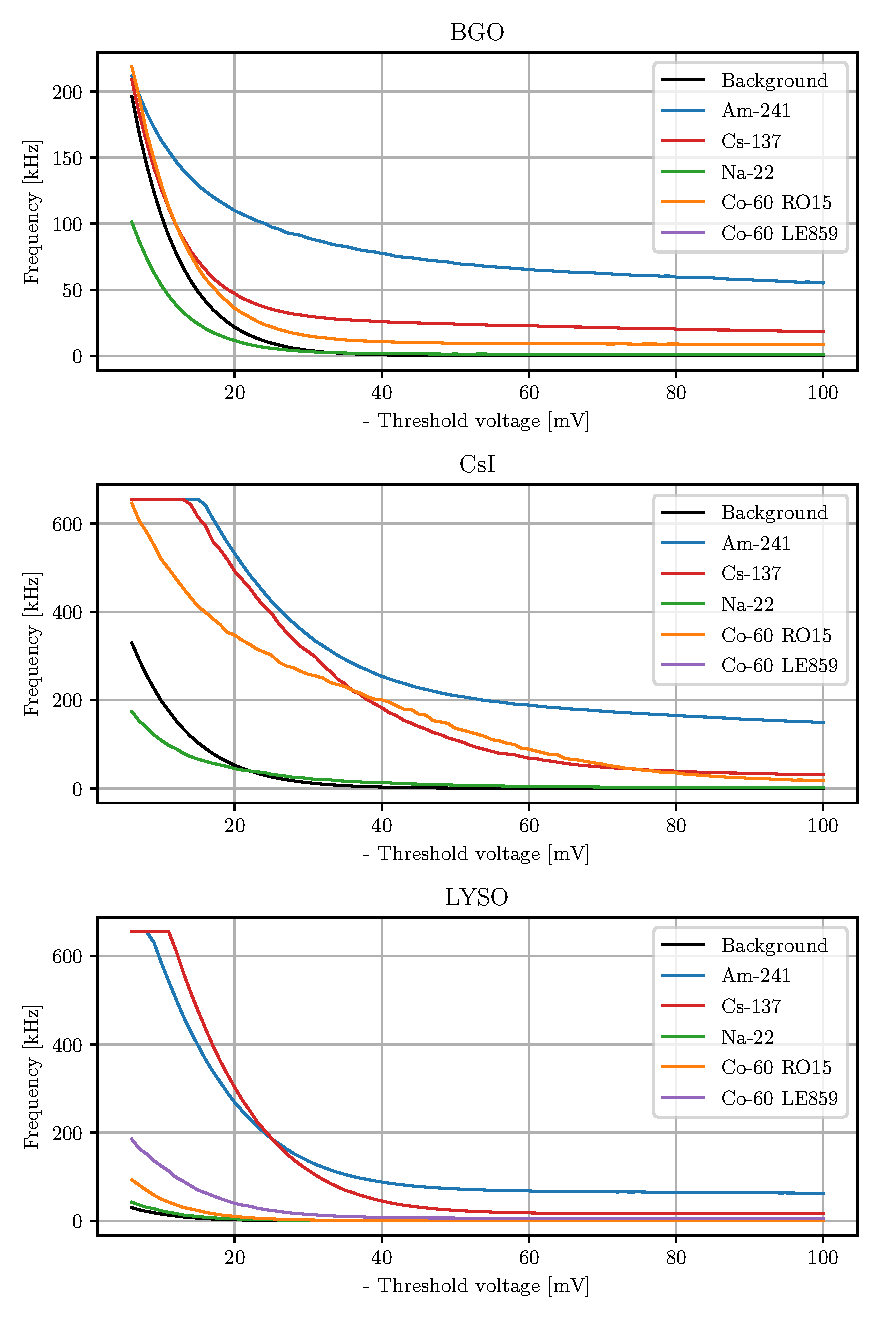
\includegraphics[height=0.88\textheight]{figures/thresholds.pdf}
    \caption{Background and signal from different sources with different crystals. The plot has been used to find the optimal threshold energy for each crystal: \SI{-70}{mV} for BGO, \SI{-80}{mV} for CsI and \SI{-40}{mV} for LYSO.}
    \label{fig:threshold}
\end{figure}

\begin{figure}[H]
    \centering
    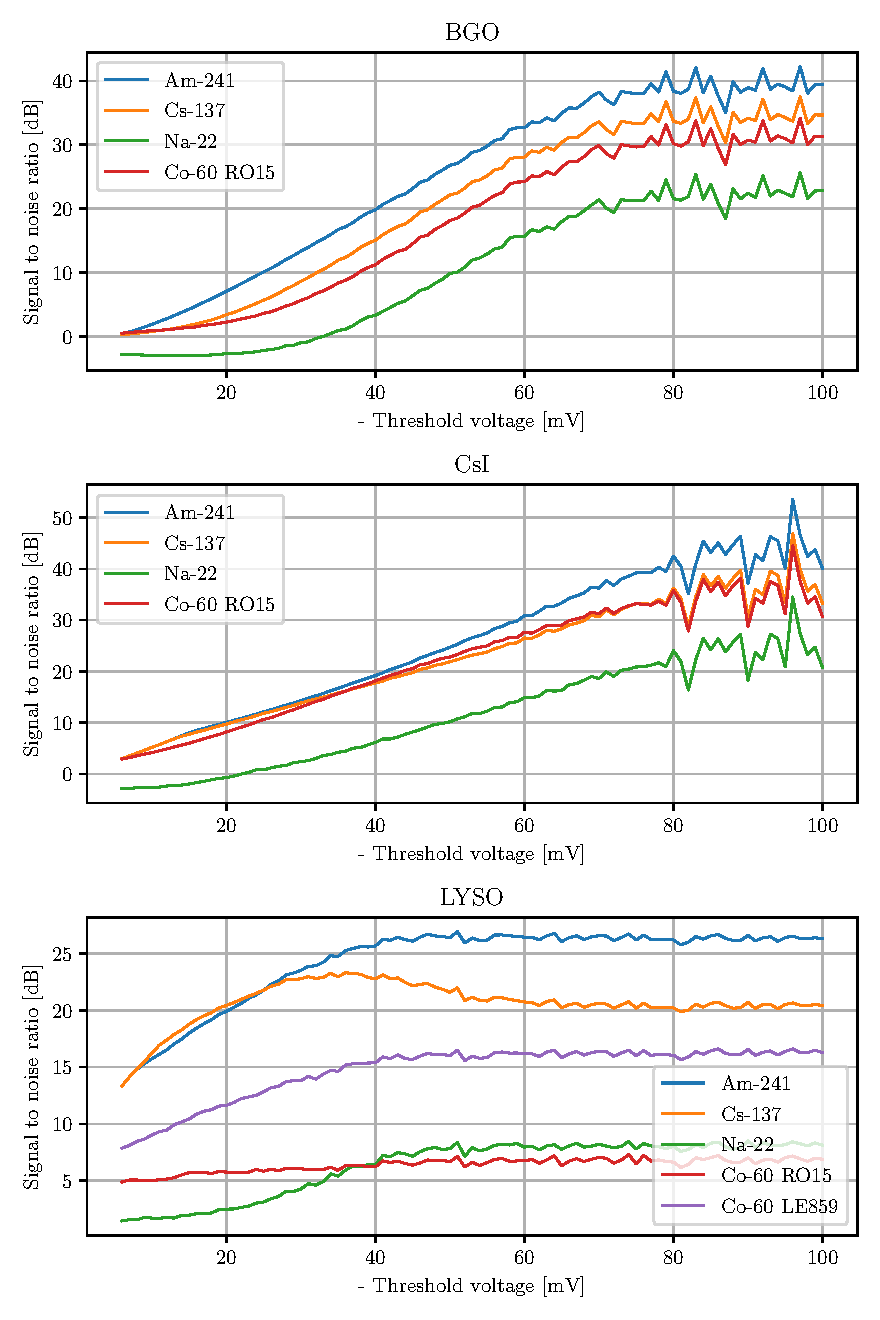
\includegraphics[height=0.88\textheight]{figures/snr.pdf}
    \caption{Signal to noise ratio of the signal from different sources with different crystals. The plot has been used to find the optimal threshold energy for each crystal: \SI{-70}{mV} for BGO, \SI{-80}{mV} for CsI and \SI{-40}{mV} for LYSO.}
    \label{fig:snr}
\end{figure}

\begin{figure}[H]
    \centering
    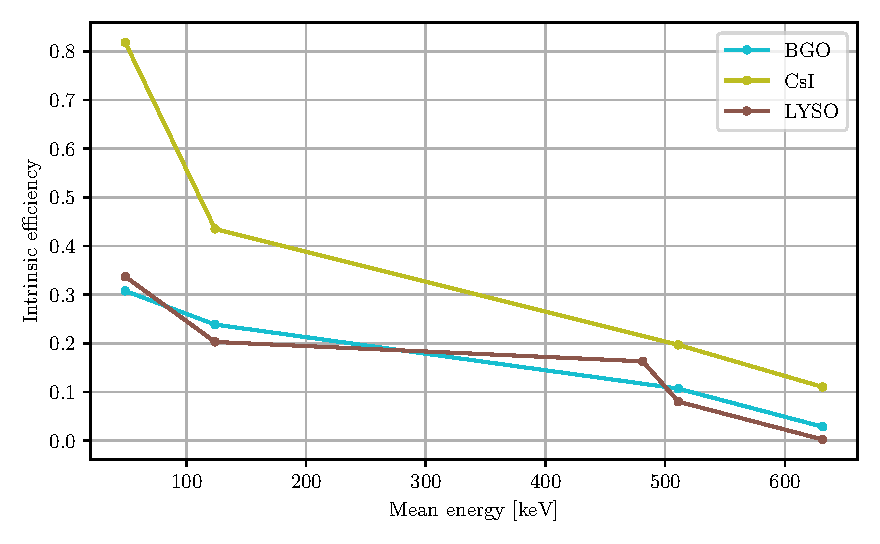
\includegraphics[width=\textwidth]{figures/efficiency.pdf}
    \caption{The intrinsic efficiency of each crystal is plotted against the mean energy of the source. Each point represents the intrinsic efficiency of a crystal with a specific source. The energy of the source is found as an average of the energies of its peaks, weighted by their height. The error bars are too small to be visible. The errors range from 0.4\% to 2\%.}
    \label{fig:efficiency}
\end{figure}

\begin{figure}[H]
    \centering
    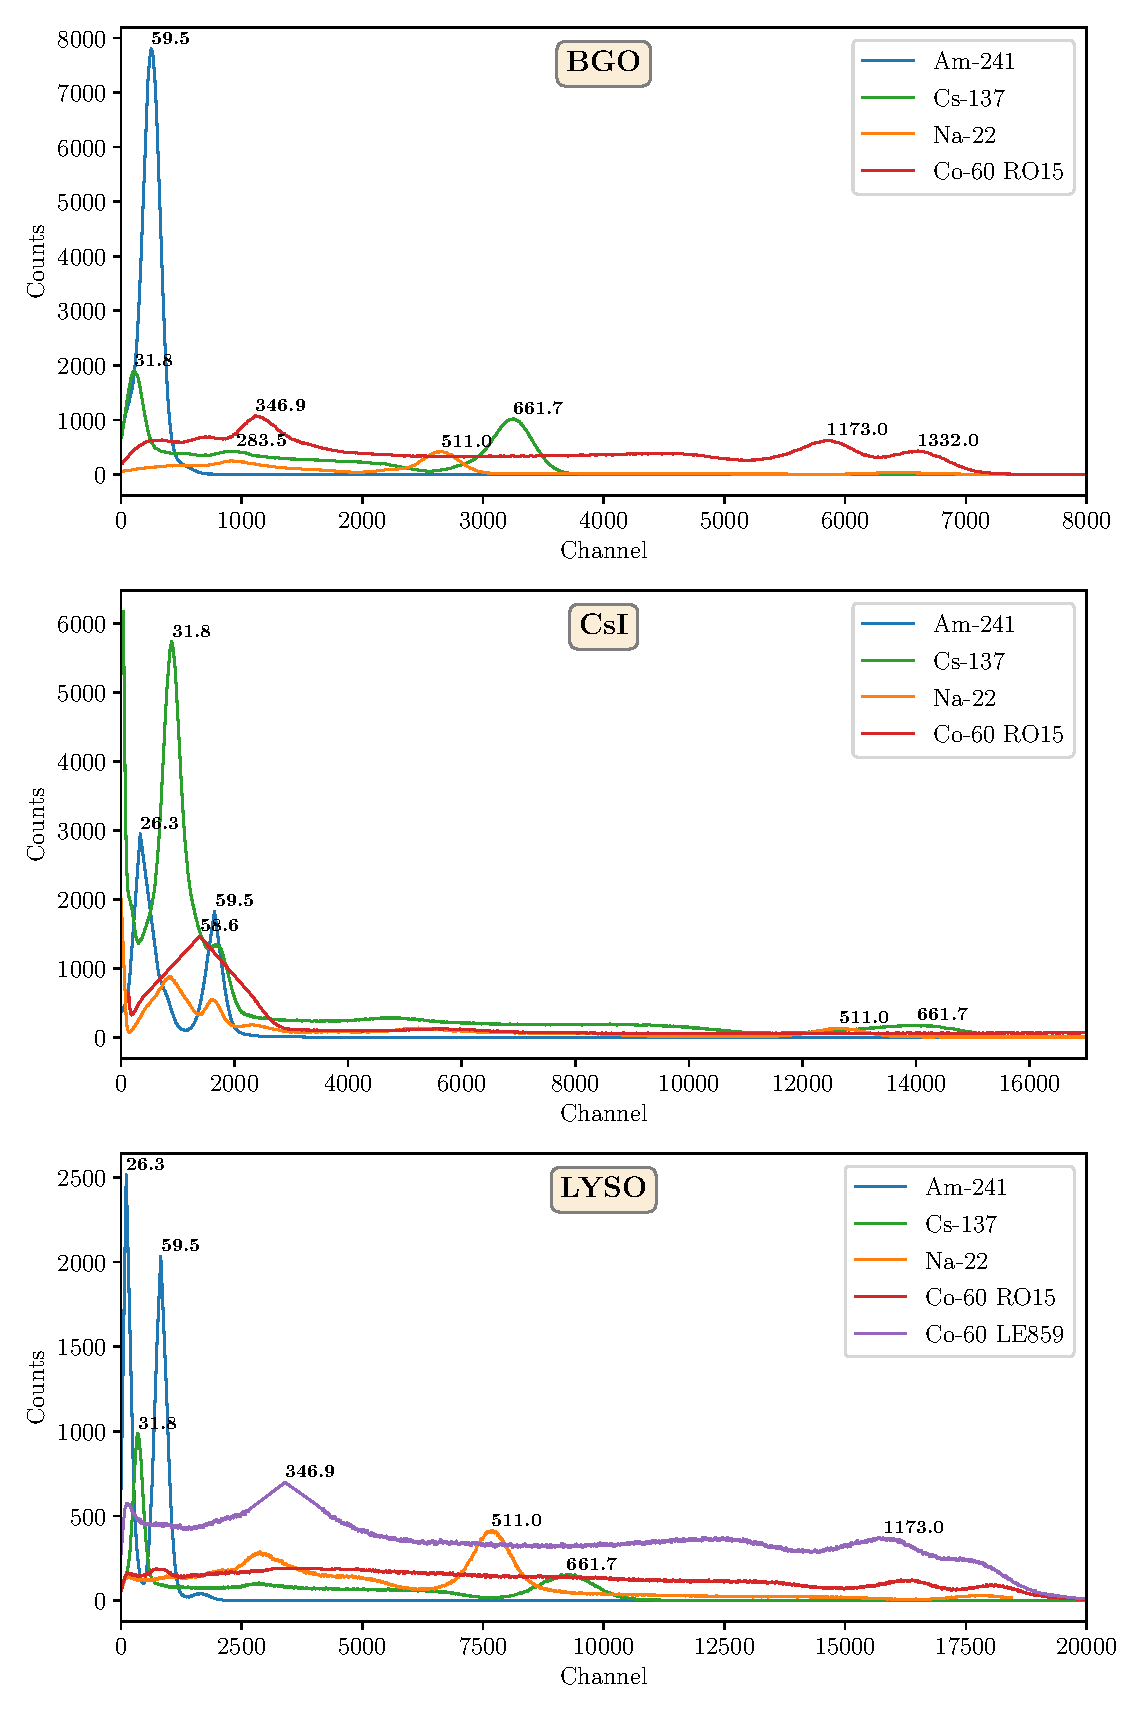
\includegraphics[height=0.9\textheight]{figures/spectra.pdf}
    \caption{Spectra of different sources. The signal has been cleaned performing a moving average. Am-241 and Co-60 peaks in CSI and Am-241 peaks in LYSO have been reconstructed approximating the signal with a straight line. The energy of the peaks are reported next to them in keV \cite{heath_scintillation_1964}.}
    \label{fig:spectra}
\end{figure}

\begin{figure}[H]
    \centering
    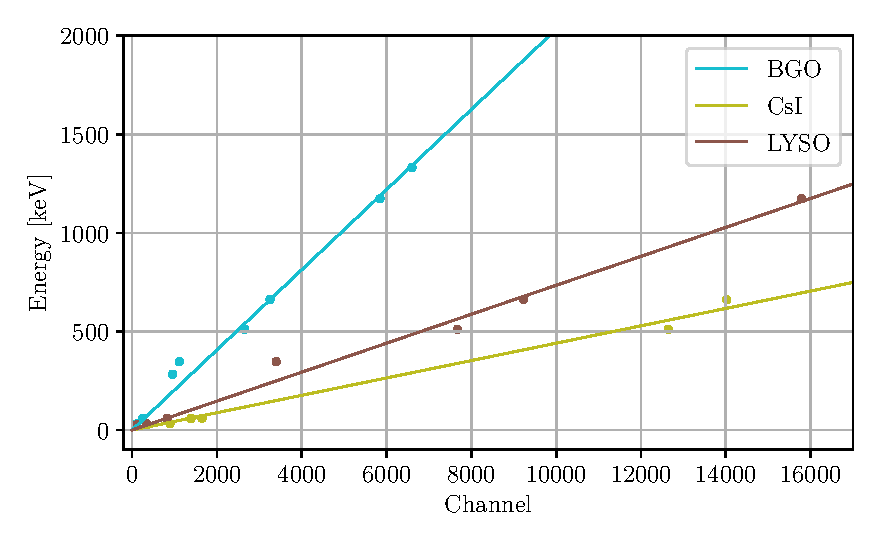
\includegraphics[width=\textwidth]{figures/calibration.pdf}
    \caption{Calibration of the spectrometer with three different crystals. Each point represent a peak of known source. The channel of the peak has been measured, while the energy has been found in literature. A linear fit ($y = mx$) forced through the 0 gives the calibration relation. The factor $m$ has been found to be \SI{0.20(10)}{keV} for BGO, \SI{0.044(16)}{keV} for CsI and \SI{0.07(2)}{keV} for LYSO.}
    \label{fig:calibration}
\end{figure}

\begin{figure}[H]
    \centering
    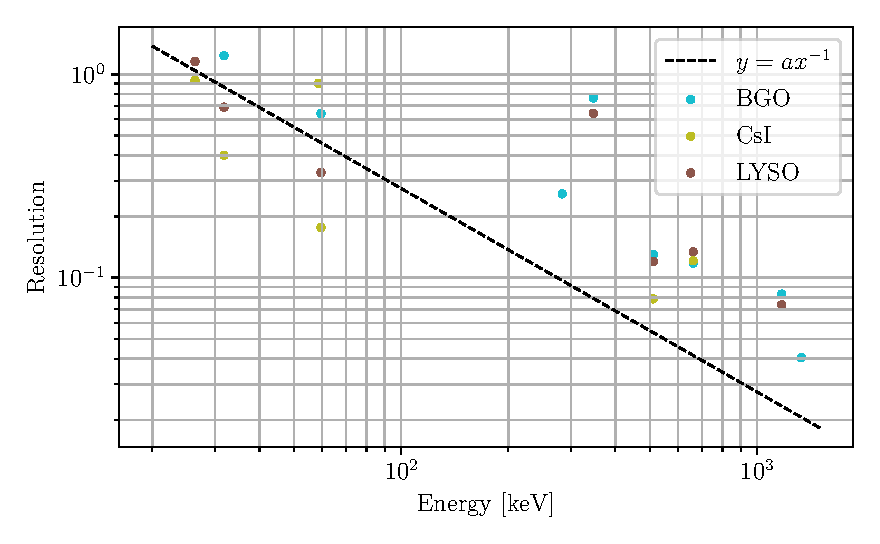
\includegraphics[width=\textwidth]{figures/resolution.pdf}
    \caption{The energy resolution of the peaks is plotted against their energy. A logarithmic scale was used for both axis. The black line is the function $y=ax^{-1}$ fitted on all the data: $a=\SI{27(3)}{keV}$.}
    \label{fig:resolution}
\end{figure}

\begin{figure}[H]
    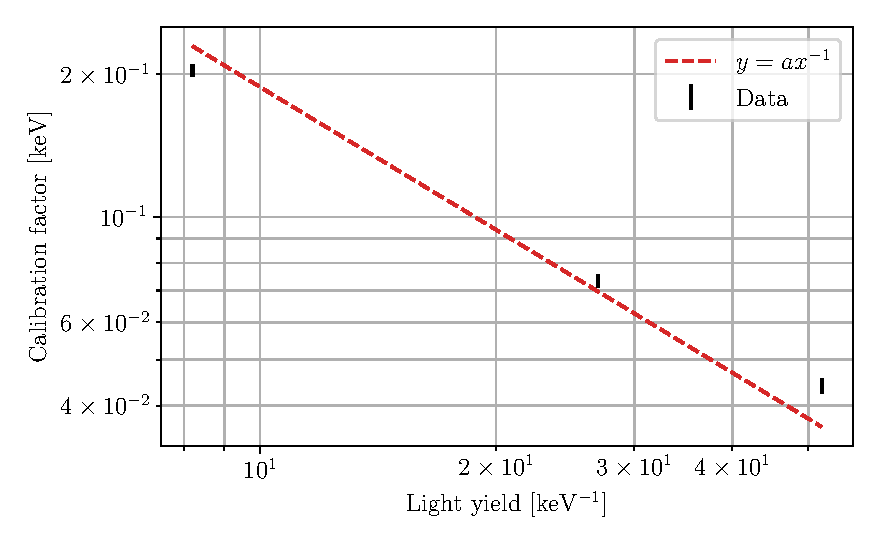
\includegraphics[width=\textwidth]{figures/light_yield.pdf}
    \caption{Calibration factors of the crystals plotted against their light yield. A logarithmic scale was used for both axis. The line red line is given by a fit of the function $y=ax^{-1}$. The parameter was found to be $a = \SI{1.87(17)}{}$.}
    \label{fig:light_yield}
\end{figure}

\section{Experimental conditions} \label{app:conditions}
\begin{table}[H]
    \centering
    \caption{Spectrometer settings and conditions}
    \label{tab:conditions}
    \begin{tabular}{llcccc}
        \toprule
        Crystal & Source      & Bias [V] & Gain [dB] & Threshold [mV] & Channel temp. [°C] \\
        \midrule
        BGO     & Am-241      & 55.0     & 40.0      & -60.0          & 25.4               \\
        BGO     & Cs-137      & 55.0     & 40.0      & -60.0          & 25.3               \\
        BGO     & Na-22       & 55.0     & 40.0      & -60.0          & 25.7               \\
        CsI     & Am-241      & 55.0     & 40.0      & -45.0          & 25.6               \\
        CsI     & Cs-137      & 55.0     & 40.0      & -75.0          & 25.6               \\
        CsI     & Na-22       & 55.0     & 40.0      & -80.0          & 25.0               \\
        LYSO    & Am-241      & 55.0     & 40.0      & -70.0          & 25.4               \\
        LYSO    & Cs-137      & 55.0     & 40.0      & -75.0          & 25.2               \\
        LYSO    & Na-22       & 55.0     & 40.0      & -25.0          & 25.3               \\
        LYSO    & Co-60 RO15  & 55.0     & 40.0      & -100.0         & 25.6               \\
        LYSO    & Co-60 LE859 & 55.0     & 40.0      & -75.0          & 25.8               \\
        \bottomrule
    \end{tabular}
\end{table}

\end{document}




